\section{PROCEDURES}

\subsection{Reference problem}
The reference problem stated is illustrated in the Fig.~\ref{fig:problem}, a panel of thickness $t$,
longitudinal length $a$, transverse length $b$,
under a given Mach number $M$ and dynamic pressure $\bar{q}$.

\begin{figure}[h!]
    \centering
    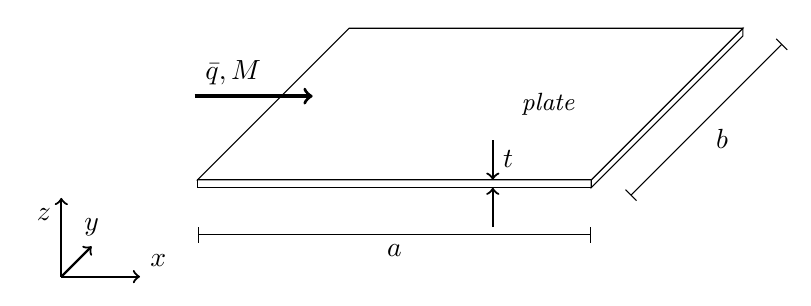
\begin{tikzpicture}
        \draw[thick,->] (-5,-2,-2)  ++(0, 0, 0) -- ++(1, 0, 0) node[anchor=south west] {$x$};
        \draw[thick,->] (-5,-2,-2)  ++(0, 0, 0) -- ++(0, 1, 0) node[anchor=north east] {$z$};
        \draw[thick,->] (-5,-2,-2)  ++(0, 0, 0) -- ++(0, 0, -1) node[anchor=south] {$y$};

        \pgfmathsetmacro{\cubex}{5}
        \pgfmathsetmacro{\cubey}{0.1}
        \pgfmathsetmacro{\cubez}{5}
        
        % \draw[black, fill=white] (2.5,0,0) ++(-\cubex/2+0.25,-\cubey-0.01,0) ++(-0.5,-0.5,0) rectangle ++(0.5,0.5,0);
        % \draw[black, fill=white] (2.5,0,0) ++(-\cubex/2+0.75,-\cubey-0.01,0) ++(-0.5,-0.5,0) -- ++(0.5,0.5,0);
        
        \draw[black, fill=white] (2.5,0,0) -- ++(-\cubex,0,0) -- ++(0,-\cubey,0) -- ++(\cubex,0,0) -- cycle;
        \draw[black, fill=white] (2.5,0,0) -- ++(0,0,-\cubez) -- ++(0,-\cubey,0) -- ++(0,0,\cubez) -- cycle;
        \draw[black, fill=white] (2.5,0,0) -- ++(-\cubex,0,0) -- ++(0,0,-\cubez) -- ++(\cubex,0,0) -- cycle;
        
        \draw[black, |-|] (2.5,-0.7,0) ++(0,0,0) -- ++(-\cubex/2,0,0)node[anchor=north] {$a$} -- ++(-\cubex/2,0,0);
        \draw[black, |-|] (3,-0.2,0) ++(0,0,0) -- ++(0,0,-\cubez/2)node[anchor=north west] {$b$} -- ++(0,0,-\cubez/2);
        
        \draw[black, thick,->] (2.5,0,0)  ++(-\cubex/4,0.5,0)node[anchor=north west]{$t$} -- ++(0,-0.5,0);
        \draw[black, thick,->] (2.5,0,0)  ++(-\cubex/4,-0.5-\cubey,0) -- ++(0,0.5,0);
        
        \draw[black, very thick, ->] (-3.5,0.1,-2.5) ++(0, 0, 0) node[anchor=south west] {$\bar{q}, M$} -- ++(1.5, 0, 0);
        
        % \draw (-1,-.4,0)node[]{\small \emph{stringer}};
        \draw (1,0,-2.5)node[]{\small \emph{plate}};
    \end{tikzpicture}
    \newline
    \caption{Panel dimensions and conditions.}
    \label{fig:problem}
\end{figure}

\subsection{Mathematical formulation}

The aerodynamic theory is a third-order Piston Theory developed by \citet{ashley_piston_1956}. As shown by \cite{pegado_metodo_2003} the Piston Theory is given by Eq.~\ref{eq:pistonTheory}, and it's third-order expansion is
given by Eq.~\ref{eq:pistonTheoryThird}.

\begin{equation}
p = p_{\infty}\Bigg[1+\frac{\gamma_{air} - 1}{2 a_{\infty}}\bigg(\frac{\partial W}{\partial t} + U_{\infty}\frac{\partial W}{\partial x}\bigg)\Bigg]^{\frac{2\gamma_{air}}{\gamma_{air}-1}}
    \label{eq:pistonTheory}
\end{equation}

\begin{equation}
p - p_{\infty} = \frac{2\bar{q}}{M}
\Bigg[
\bigg(\frac{1}{U_{\infty}}
\frac{\partial W}{\partial t} + \frac{\partial W}{\partial x}\bigg)
+
\frac{\gamma_{air}+1}{4}M
\bigg(\frac{1}{U_{\infty}}
\frac{\partial W}{\partial t} + \frac{\partial W}{\partial x}\bigg)^2
+
\frac{\gamma_{air}+1}{12}M^2
\bigg(\frac{1}{U_{\infty}}
\frac{\partial W}{\partial t} + \frac{\partial W}{\partial x}\bigg)^3
\Bigg]
    \label{eq:pistonTheoryThird}
\end{equation}

Where $p$ is the aerodynamic pressure in the surface of the plate, $p_{\infty}$ is the aerodynamic pressure of the undisturbed flow, $\gamma_{air}$ is the ratio of the air specific heat constants, $U_{\infty}$ is the velocity of the undisturbed flow, $a_{\infty}$ is the velocity of sound in the undisturbed flow and $W$ is the vertical plate displacement.

\subsection{Numerical modeling}

The aerodynamic panel is discretized in chord-wise elements \emph{CAERO5} with element property \emph{PAERO5}, each element has user defined number of span-wise strips, as illustrated in Fig. \ref{fig:problem-discrete}. 

\input{sections/model-discrete.tex}

Aerodynamic and structural models can be linked through a surface spline \emph{SPLINE1} or linear spline \emph{SPLINE2} elements.
\citet{siemens_nx_2014} indicates that rigid chord condition must be satisfied for the splines, so attachment flexibility is not allowed.
It must be specified the number of aerodynamic elements for the geometry and which set of structural nodes will be interpolated through the spline for each aerodynamic element.

As part of the solution sequence, it must be specified the parameter to run a modal analysis, which consist of the number of modes to search, the range of frequencies and the method.

It also must be specified the solution method for the aeroelastic sequence. The currently available methods are the \emph{K}, \emph{KE}, \emph{PK} and the \emph{PK-NL}, the last two are the most common used.

The flow conditions must be specified for Mach numbers, velocities and air densities, also the analysis properties of reduced frequencies and the thickness integrals corresponding the shape of the panel cross section. The values of Mach of known good correspondence of the used aerodynamic theory are $2.5 < M < 5$. To simulate a gap under the plane (no air flow) is used a air density ratio of $\frac{1}{2}$.
\cite{siemens_nx_2014}

\subsection{Solution Sequence}

Having the structural model ready and defined the problem set, the user is prompted in the Femap's interface to insert the corners of the aerodynamic panel, the number of elements span-wise and chord-wise and the structural grid nodes for each aerodynamic element.
% The model is shown at the Fig.\ref{fig:model}.

% \begin{figure}[h!]
%     \centering
%     \includegraphics[scale=0.5]{figures/undef model.png}
%     \caption{FEM model.}
%     \label{fig:model}
% \end{figure}

The the aeroelastic solution card is generated and executed in the NASTRAN solver.
The results are then plotted in \emph{Vg} and \emph{Vf} graphics for each mode, as well the complex eigenvalues.
The result set is imported in Femap, enabling the visualization of the result.